\documentclass{jsarticle}
\usepackage[dvipdfmx]{graphicx}
\usepackage{here}
\usepackage{listings,jlisting}
\title{\Huge 確率論・統計学 中間課題}

\author{\Large ******* ****}
\date{\today}
\begin{document}
\maketitle

\newpage

\section{課題1}

以下に、RStudioコンソールでの入出力を記載する。

\begin{lstlisting}[language=r]
> di <- read.table('DI4domain.csv', sep=',', header=T)
> hist(di$Koyou, col='green')
\end{lstlisting}

出力された画像が図\ref{ex1}である。

\begin{figure}[H]
 \centering
   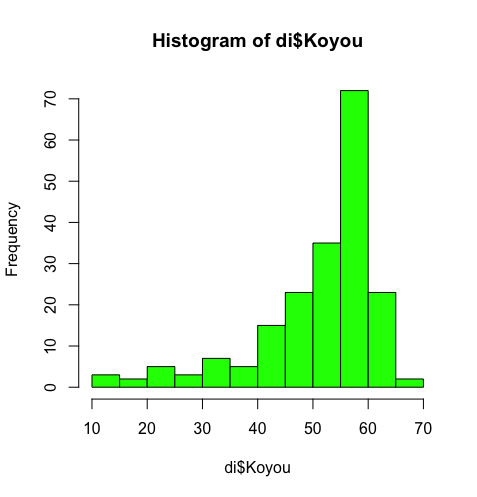
\includegraphics[width=100mm]{figures/ex1.png}
 \caption{ヒストグラム}
 \label{ex1}
\end{figure}

\section{課題2}

\subsection{平均値の最大・最小地域の同定}

以下に、RStudioコンソールでの入出力を記載する。この出力より、DI平均値が最も高いのはOkinawa、最も低いのはKanto.north.だということがわかる。

\begin{lstlisting}[language=r]
> di <- read.table('DI4area.csv', sep=',', header=T)
> di_mean <- c()
> for (x in 3:16) {
+   di_mean[names(di)[x]] <- mean(di[, x])
+ }
> which.max(di_mean)
Okinawa
     15
> which.min(di_mean)
Kanto.north.
           5 
\end{lstlisting}

\subsection{箱ひげ図の描画}

以下に、RStudioコンソールでの入出力を記載する。ただし、変数diは上で定義したものである。

\begin{lstlisting}[language=r]
> boxplot(di$Okinawa, di$Kanto.north., names=c('Okinawa', 'Kanto.north.'))
\end{lstlisting}

出力された箱ひげ図が図\ref{ex2}である。

\begin{figure}[H]
 \centering
   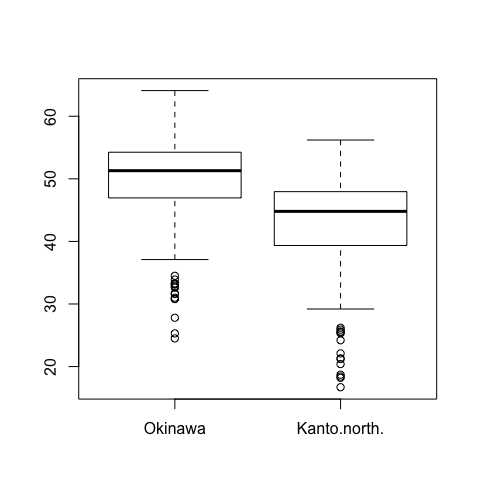
\includegraphics[width=100mm]{figures/ex2.png}
 \caption{箱ひげ図}
 \label{ex2}
\end{figure}

\section{課題3}

\subsection{ピアソン相関係数の最小地域の同定}

以下に、RStudioコンソールでの入出力を記載する。この出力より、ピアソン相関係数が最も低いのはOkinawaだということがわかる。

\begin{lstlisting}[language=r]
> di_area <- read.table('DI4area.csv', sep=',', header=T)
> di_domain <- read.table('DI4domain.csv', sep=',', header=T)
> di_cor <- c()
> for (x in 3:16) {
+   di_cor[names(di)[x]] <- cor(di_area[, x], di_domain$Kigyo)
+ }
> which.min(di_cor)
Okinawa
     14 
\end{lstlisting}

\subsection{散布図の描画}

以下に、RStudioコンソールでの入出力を記載する。ただし、変数di\_area、di\_domainは上で定義したものである。

\begin{lstlisting}[language=r]
> plot(di_area$Okinawa, di_domain$Kigyo)
\end{lstlisting}

出力された散布図が図\ref{ex3}である。

\begin{figure}[H]
 \centering
   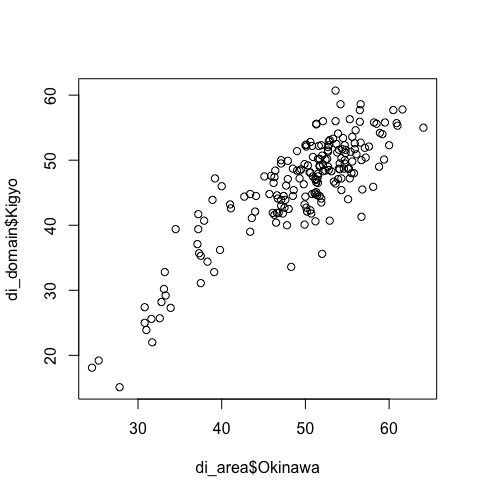
\includegraphics[width=100mm]{figures/ex3.png}
 \caption{散布図}
 \label{ex3}
\end{figure}

\section{課題4}
\subsection{企業関連DIデータと乱数列のピアソン相関係数}

以下に、RStudioコンソールでの入出力を記載する。

\begin{lstlisting}[language=r]
> di <- read.table('DI4domain.csv', sep=',', header=T)
> cors <- c()
> rands <- c()
> for (x in 1:1000) {
+   rand <- runif(195, min=0, max=100)
+   rands <- c(rands, rand)
+   cor <- cor(di$Kigyo, rand)
+   cors <- c(cors, cor)
+ }
> hist(cors)
\end{lstlisting}

出力されたヒストグラムが図\ref{ex4}である。

\begin{figure}[H]
 \centering
   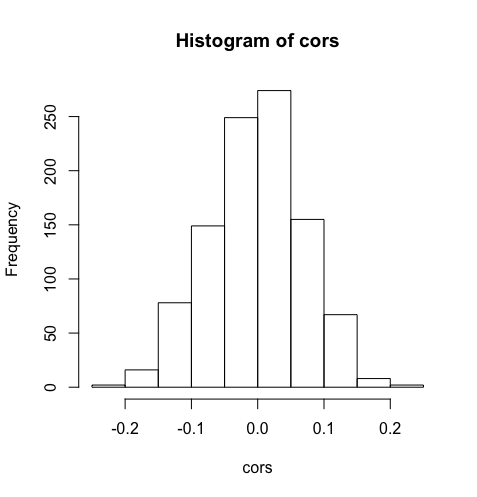
\includegraphics[width=100mm]{figures/ex4.png}
 \caption{ヒストグラム}
 \label{ex4}
\end{figure}

\subsection{相関が最大値のものについて、線形回帰分析}

以下に、RStudioコンソールでの入出力を記載する。ただし、di、cors、randsは上で定義したものである。出力より、切片$46.397909$、傾き$-0.005949$だとわかる。

\begin{lstlisting}[language=r]
> which.max(cors)
[1] 426
> rands_matrix <- matrix(rands, nrow=1000, ncol=195)
> result <- lm(di$Kigyo ~ rands_matrix[426,])
> summary(result)

Call:
lm(formula = di$Kigyo ~ rands_matrix[426, ])

Residuals:
    Min      1Q  Median      3Q     Max 
-31.169  -2.945   1.517   5.122  14.465 

Coefficients:
                     Estimate Std. Error t value Pr(>|t|)    
(Intercept)         46.397909   1.137230  40.799   <2e-16 ***
rands_matrix[426, ] -0.005949   0.019912  -0.299    0.765    
---
Signif. codes:  0 ‘***’ 0.001 ‘**’ 0.01 ‘*’ 0.05 ‘.’ 0.1 ‘ ’ 1

Residual standard error: 8.018 on 193 degrees of freedom
Multiple R-squared:  0.0004623,	Adjusted R-squared:  -0.004717 
F-statistic: 0.08927 on 1 and 193 DF,  p-value: 0.7654

\end{lstlisting}

\section{課題5}

DI4domain.csvから、2016年1月から2017年12月までのデータのみ切り出したものを作成し、DI4domain\_16-17.csvとして保存した。s-Statより、「労働力調査 基本集計 全都道府県 全国 月次」統計の「産業,雇用形態別雇用者数(2013年1月~)」表をCSV形式でダウンロードし、DI4domain\_16-17.csvのような形式に整形した。これをlabor\_16-17.csvとして保存した。

\subsection{DIと雇用者数の相関係数}

以下に、RStudioコンソールでの入出力を記載する。この出力より、DIと雇用者(worker)数の相関が強く、相関係数はおよそ$0.85$ということがわかる。

\begin{lstlisting}[language=r]
> di <- read.table('DI4domain_16-17.csv', sep=',', header=T)
> labor <- read.table('labor_16-17.csv', sep=',', header=T)
> cors <- c()
> for (x in 2:9) {
+   cors[names(labor)[x]] <- cor(labor[, x], di$Total)
+ }
> cors
worker    employee     regular   irregular    parttime   temporary    contract   parttime2 
0.85053398  0.83442635  0.68079522  0.76881785  0.73475050  0.17279154  0.34709905 -0.02946126 
\end{lstlisting}

\subsection{折れ線グラフの描画}

以下に、RStudioコンソールでの入出力を記載する。ただし、di、laborは上で定義したものである。

\begin{lstlisting}[language=r]
> par(oma=c(0, 0, 0, 2))
> plot(di$Total, type='l', ylim=c(40, 56), axes=F)
> axis(1, at=1:24, di$Month)
> axis(2)
> par(new=T)
> plot(labor$worker, type='l', col='red', axes=F,
+   ylim=c(5650, 5900), xlab='', ylab='')
> mtext('labor$worker', side=4, line=3)
> axis(4)
> box()
> legend('topleft', legend=c('di$Total', 'labor$worker'),
+   col=c('black', 'red'), lty=1)
\end{lstlisting}

出力された折れ線グラフが図\ref{ex5}である。なお、雇用者の単位は(万人)である。

\begin{figure}[H]
 \centering
   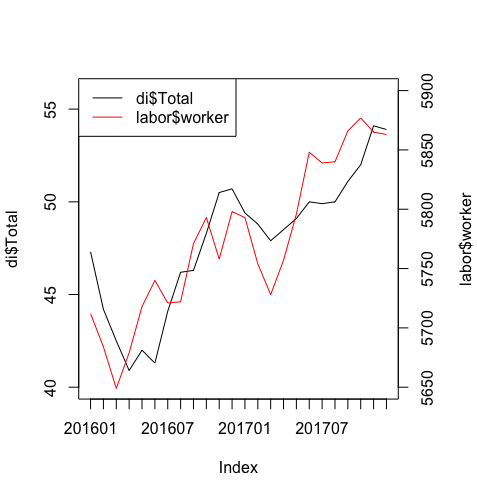
\includegraphics[width=100mm]{figures/ex5.png}
 \caption{折れ線グラフ}
 \label{ex5}
\end{figure}

\subsection{議論}

相関係数が1に近いことから、DIと雇用者数は正の相関関係にあると言える。また、DIの指標の中に常用雇用指数が含まれていることから、雇用者数とDIは因果関係にあると言える。

\end{document}
